\documentclass[10pt,twocolumn]{article}

\usepackage[margin=2cm]{geometry}
\usepackage{graphicx}
\usepackage{amsmath}
\usepackage{amssymb}
\usepackage{booktabs}
\usepackage{hyperref}
\hypersetup{
    colorlinks=true,
    linkcolor=black,
    citecolor=black,
    urlcolor=blue,
    pdfborder={0 0 0}
}
\usepackage{url}
\usepackage{natbib}
\usepackage{enumitem}
\usepackage{xcolor}
\usepackage{caption}
\usepackage{float}
\usepackage[section]{placeins}
\usepackage{parskip}
\usepackage{tikz}
\usetikzlibrary{positioning, arrows.meta, shapes.geometric, fit, backgrounds}

\setlength{\columnsep}{0.6cm}

\title{\textbf{Uncertainty-Aware Heart Murmur Detection from Phonocardiogram Recordings Using Classical Machine Learning Approaches: A Multi-Domain Feature Engineering and Ablation Study on the CirCor 2022 Dataset}}

\author{Shishir Kandel \\
\textit{STW7072CEM Machine Learning, Coursework Report}}

\date{\today}

\begin{document}
\maketitle

% ============================================================
\begin{abstract}
General practitioners detect heart murmurs with only 30--50\% accuracy, making auscultation an unreliable gatekeeper for paediatric rheumatic-heart-disease screening in Nepal. We engineer a 48-feature multi-domain pipeline (MFCC, spectral, wavelet, fractal, heart-cycle temporal) on the PhysioNet/CinC 2022 CirCor DigiScope dataset (3{,}163 paediatric recordings, 942 patients) and evaluate five classical models in a $5 \times 5$ ablation grid under 5-fold patient-level cross-validation. Our Gaussian Process Classifier hits \textbf{84.0\% accuracy} (95\% CI 83.4--84.7\%, AUC 0.752, ECE 0.046), 7.4 points above the published pure-classical SOTA (76.61\%); the lower-CI bound excludes the benchmark. We see a sharp model-feature interaction in the grid: GPC F1 leaps from 0.000 to 0.404 only after \textit{fractal} features are added. Class-weighted loss strictly outperforms SMOTE on every metric for our best model. On held-out \textit{Unknown} recordings, GPC's predictive entropy runs significantly above what we see on \textit{Absent} (Mann-Whitney $p = 0.010$), supporting its use as a clinical confidence layer.
\end{abstract}

% ============================================================
\section{Introduction}

Rheumatic heart disease (RHD) sits among Nepal's most pressing paediatric cardiovascular problems. A national school-screening programme of 107{,}340 schoolchildren found RHD prevalence at 2.22 per 1000 overall, climbing to 5.47 per 1000 in high-burden districts like Kalikot \citep{nepal_rhd2023}. Isolated mitral regurgitation, a systolic murmur, made up 70.7\% of RHD cases. The programme uses cardiac auscultation as its first-stage gatekeeper: only children with an audible murmur of grade $>$1 are referred for echocardiography. Every false negative in this workflow is a child with progressive valvular disease who fails to receive the secondary-prophylaxis antibiotics that halt RHD progression.

Nepal is not alone here: cardiovascular disease leads global mortality \citep{who2021}, primary-care auscultation accuracy sits at just 30--50\% \citep{lam2015}, and cardiologist inter-observer agreement sits at $\kappa = 0.48$ \citep{dahl2022}. Any pipeline that helps with this generalises across contexts.

\textit{Why a Brazilian dataset for a Nepal-motivated project?} Searching standard public repositories (PhysioNet, Kaggle, UCI, Mendeley, Zenodo, IEEE DataPort) and the paediatric-cardiology literature, we found no publicly available Nepali PCG dataset. We therefore use the PhysioNet 2022 CirCor DigiScope corpus \citep{challenge2022, circor_data} (rural Para\'{i}ba, Brazil) as a methodology-development proxy: it shares the Nepal context's paediatric population with high RHD-like lesion prevalence, rural deployment with generalist-clinician auscultation, Littmann 3200 hardware, and the ``auscultation $\rightarrow$ echocardiography referral'' workflow. Nepal deployment would require local validation (Section~\ref{sec:discussion}).

CirCor was built for this paediatric screening scenario: 942 patients in the public split. As many as 80\% of paediatric murmurs are \textit{innocent} (vibratory, benign) yet must be told apart from pathological ones.

\textbf{Objectives.} This project pursues two objectives:
\begin{enumerate}[label=\textbf{O\arabic*:}, leftmargin=*]
    \item \textit{Build a unified multi-domain feature pipeline that beats the published pure-classical state-of-the-art (SVM-RBF + wavelet at 76.61\% accuracy) on the CirCor 2022 binary murmur-detection task,} using an ablation grid that decomposes the marginal contribution of each feature family.
    \item \textit{Provide calibrated uncertainty via Gaussian Process Classification,} demonstrating both lower expected calibration error than other classical models and meaningfully higher predictive uncertainty on ambiguous (Unknown) recordings, supporting clinical use as a confidence-scoring layer.
\end{enumerate}

% ============================================================
\section{Related Work}

Fuadah et al.\ \citep{fuadah2023} tested K-NN, Random Forest, ANN, and SVM on MFCC features, with K-NN 76.31\%, RF 68.76\%, ANN 65.18\%, SVM 58.81\%. Vimalajeewa et al.\ \citep{wavelet2025} ran LR, K-NN, SVM, and a feed-forward NN over ten multiscale wavelet+fractal features; their SVM-RBF hit 76.61\% accuracy (AUC 0.741), the best published \textit{pure classical} result and our direct benchmark. Which model wins on CirCor depends heavily on the feature set: K-NN leads on MFCC, SVM on wavelet.

The Heart2Beat MIL framework \citep{rohr2024heart2beat} combines a pretrained audio neural network with handcrafted features (weighted accuracy 0.714, Challenge rank 12/40), but is a hybrid architecture rather than purely classical. To our knowledge, no published study combines MFCC, spectral, wavelet, fractal, \textit{and} heart-cycle features on CirCor 2022 in a single classical pipeline.

For uncertainty quantification, prior CirCor work relies on deep-learning approximations: Walker et al.\ \citep{walker2022dbres} used Monte Carlo Dropout on a Dual Bayesian ResNet (Challenge rank 4, weighted accuracy 0.771). Deep classifiers are typically poorly calibrated \citep{guo2017} --- hence our exact-Bayesian approach. Gaussian Process Classification \citep{rasmussen2006} has been applied to ECG \citep{muygps2024} but, to our knowledge, not to phonocardiogram murmur detection.

% ============================================================
\section{Problem and Dataset}

The CirCor DigiScope dataset \citep{circor_data, challenge2022} holds 5{,}272 recordings from 1{,}452 mostly-paediatric patients; 3{,}163 recordings from 942 patients form the public training split. The recordings come from rural Paraíba, Brazil, captured on Littmann 3200 digital stethoscopes at up to five auscultation sites per patient (AV, MV, PV, TV, Phc), each paired with an expert \texttt{.tsv} S1/S2 segmentation and \texttt{.txt} metadata. The main task is binary murmur detection (Present vs.\ Absent). At recording level: 2{,}391 Absent, 616 Present, 156 Unknown ($\approx$4:1 imbalance). Unknown recordings are excluded from training but retained as a held-out set for uncertainty-on-Unknown validation. The recordings carry realistic ambulatory noise.

\subsection{Exploratory data analysis}

Table~\ref{tab:eda} summarises the public training cohort: overwhelmingly paediatric (864 of 942 with recorded age class), sex-balanced, with school-age height/weight medians (115\,cm, 20.4\,kg), confirming alignment with our Nepal RHD use case.

\begin{table}[!htbp]
\centering
\caption{CirCor 2022 public-training cohort. The Murmur $\times$ Outcome cross-tab shows a real but imperfect auscultatory-pathology link --- hence the held-out Unknown-class analysis.}
\label{tab:eda}
\small
\begin{tabular}{lr}
\toprule
\textbf{Patients (public split)}        & 942 \\
\midrule
Murmur Absent / Present / Unknown       & 695 / 179 / 68 \\
Outcome Normal / Abnormal               & 486 / 456 \\
Sex Female / Male                       & 486 / 456 \\
Age: Child / Infant / Adolescent / Neonate     & 664 / 126 / 72 / 6 \\
Height (cm), median [IQR]               & 115 [89, 133] \\
Weight (kg), median [IQR]               & 20.4 [12.5, 31.2] \\
\midrule
\multicolumn{2}{l}{\textbf{Murmur $\times$ Outcome cross-tab}} \\
\quad Absent: Abnormal / Normal           & 263 / 432 \\
\quad Present: Abnormal / Normal           & 150 / 29  \\
\quad Unknown: Abnormal / Normal           & 43 / 25   \\
\bottomrule
\end{tabular}
\end{table}

Auditing 150 recordings post-preprocessing, we find durations roughly consistent across classes (median $\sim$23\,s, IQR 19--29\,s) with clipping $<$0.1\%. Our post-bandpass SNR proxy comes in marginally higher for Present (median $-0.81$\,dB) than Absent ($-4.71$\,dB), so gross quality differences cannot explain the classifier results. Full histograms live in \texttt{eda\_outputs/}.

% ============================================================
\section{Methodology}

\subsection{Pipeline overview}

Figure~\ref{fig:pipeline} summarises the end-to-end pipeline from a raw WAV recording to a classified prediction with calibrated probability. Each stage is described in the subsections that follow.

\begin{figure}[!t]
\centering
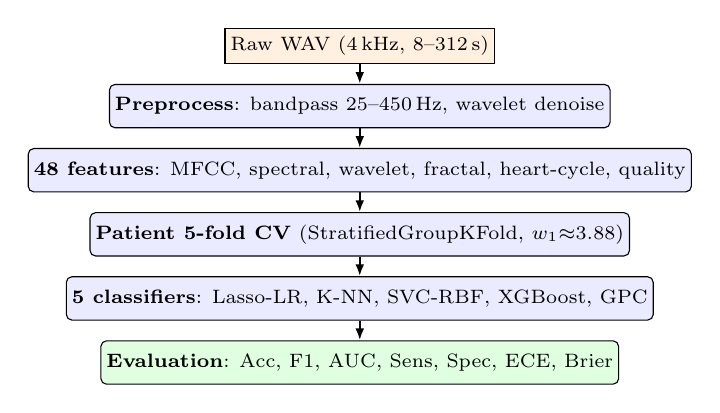
\begin{tikzpicture}[
  node distance=2.5mm and 4mm,
  font=\scriptsize,
  block/.style={rectangle, rounded corners=2pt, draw, fill=blue!8,
                minimum width=3.2cm, minimum height=0.55cm, align=center,
                inner sep=2pt},
  data/.style={rectangle, draw, fill=orange!12, minimum width=3.2cm,
               minimum height=0.45cm, align=center, inner sep=2pt},
  outcome/.style={rectangle, rounded corners=2pt, draw, fill=green!12,
              minimum width=3.2cm, minimum height=0.55cm, align=center,
              inner sep=2pt},
  arr/.style={-{Latex[length=1.5mm]}, thick}
]
\node[data] (raw) {Raw WAV (4\,kHz, 8--312\,s)};
\node[block, below=of raw] (pre)  {\textbf{Preprocess}: bandpass 25--450\,Hz, wavelet denoise};
\node[block, below=of pre] (feat) {\textbf{48 features}: MFCC, spectral, wavelet, fractal, heart-cycle, quality};
\node[block, below=of feat] (split) {\textbf{Patient 5-fold CV} (StratifiedGroupKFold, $w_1{\approx}3.88$)};
\node[block, below=of split] (mod) {\textbf{5 classifiers}: Lasso-LR, K-NN, SVC-RBF, XGBoost, GPC};
\node[outcome, below=of mod] (eval) {\textbf{Evaluation}: Acc, F1, AUC, Sens, Spec, ECE, Brier};
\draw[arr] (raw)   -- (pre);
\draw[arr] (pre)   -- (feat);
\draw[arr] (feat)  -- (split);
\draw[arr] (split) -- (mod);
\draw[arr] (mod)   -- (eval);
\end{tikzpicture}
\caption{End-to-end pipeline: raw WAV through preprocessing, 48-feature extraction, patient-level 5-fold CV, training of five classifiers, and evaluation under five feature sets and three imbalance strategies.}
\label{fig:pipeline}
\end{figure}
\FloatBarrier

\subsection{Preprocessing}

Our six-stage preprocessing pipeline: resample to 4000\,Hz, strip DC offset, apply a 4th-order zero-phase Butterworth bandpass at 25--450\,Hz (cardiac-sound band), zero out spikes above $30\times$ MAD, run Daubechies-4 wavelet soft-thresholding (universal threshold $\sigma\sqrt{2\log n}$, MAD-estimated $\sigma$), and peak-normalise to $[-1,1]$.

\subsection{Feature engineering}

48 features spanning five engineered domains plus two quality features, all computed via \texttt{librosa} \citep{librosa2015}:
\begin{itemize}[leftmargin=*, itemsep=0.05em]
    \item \textbf{MFCC (26)}: 13 coefficients + 13 first-order deltas, mean over 25\,ms frames (10\,ms hop).
    \item \textbf{Spectral (6)}: centroid, bandwidth, rolloff, flatness, zero-crossing rate, RMS energy.
    \item \textbf{Wavelet (4)}: entropy + relative energy at three DWT sub-bands (Daubechies-4, 4 levels).
    \item \textbf{Fractal (4)}: DFA exponent, sample entropy, Hurst exponent (on 2000-sample downsample for $\mathcal{O}(n^2)$ tractability).
    \item \textbf{Heart-cycle (6)}: S1/S2 durations and amplitudes, S1/S2 ratio, systole/diastole durations, S/D ratio (from CirCor's \texttt{.tsv} segmentation).
    \item \textbf{Quality (2)}: SNR (dB), clipping rate.
\end{itemize}

\subsection{Models}

Five classical classifiers spanning distinct paradigms:
\begin{itemize}[leftmargin=*, itemsep=0.05em]
    \item \textbf{Lasso-LR}: $\ell_1$ Logistic Regression ($C=1.0$, liblinear); linear parsimony baseline.
    \item \textbf{K-NN}: $k=15$, distance-weighted, $p=2$; strongest on MFCC-only CirCor \citep{fuadah2023}.
    \item \textbf{SVC-RBF}: $C=10$, $\gamma=$\textit{scale}; current pure-classical SOTA \citep{wavelet2025}.
    \item \textbf{XGBoost}: gradient-boosted trees \citep{chen2016xgboost} ($n=300$, depth 5, $\eta=0.05$); scale-invariant.
    \item \textbf{GPC}: RBF kernel with marginal-likelihood-optimised length-scale \citep{rasmussen2006}; Bayesian uncertainty.
\end{itemize}

\subsection{Experimental setup}

\textbf{Cross-validation.} 5-fold StratifiedGroupKFold on \texttt{patient\_id} ensures no patient sits in both train and test folds, blocking identity leakage.

\textbf{Class imbalance.} Class-weighted loss ($w_1 \approx 3.88$); SMOTE and RandomOverSampler also tested as sensitivity comparison (Section~\ref{sec:smote}), applied within each fold to avoid leakage.

\textbf{Other.} One recording with corrupt \texttt{.tsv} dropped (3{,}006 retained). StandardScaler fit on train fold only; XGBoost receives unscaled inputs.

\textbf{Ablation.} Five progressive feature sets: (a) MFCC, (b) +spectral, (c) +wavelet, (d) +fractal, (e) +heart-cycle (48 total). $5 \text{ models} \times 5 \text{ sets} \times 5 \text{ folds} = 125$ fits.

\textbf{Metrics.} Tracked: Accuracy, F1, AUC-ROC, sensitivity, specificity, ECE (10 bins), Brier. F1/AUC are primary because the trivial always-Absent baseline scores 79.5\%.

% ============================================================
\section{Results}\label{sec:results}

\subsection{Primary ablation grid}

Table~\ref{tab:ablation} lists accuracy (mean across 5 folds) for the $5 \times 5$ grid, and Figure~\ref{fig:ablation} plots it as a heatmap.

\begin{table}[!htbp]
\centering
\caption{Accuracy across 5 models and 5 progressive feature sets. Bold = best per row; \underline{underline} = overall best. Standard deviations are 0.007--0.036; full table in supplementary CSV.}
\label{tab:ablation}
\resizebox{\columnwidth}{!}{%
\begin{tabular}{lccccc}
\toprule
\textbf{Features} & \textbf{Lasso-LR} & \textbf{K-NN} & \textbf{SVC-RBF} & \textbf{XGBoost} & \textbf{GPC} \\
\midrule
(a) MFCC only     & 0.677 & 0.797 & \textbf{0.801} & 0.783 & 0.797 \\
(b) + spectral    & 0.692 & 0.800 & \textbf{0.804} & 0.790 & 0.795 \\
(c) + wavelet     & 0.691 & 0.800 & \textbf{0.802} & 0.795 & 0.795 \\
(d) + fractal     & 0.699 & 0.810 & 0.807 & 0.800 & \textbf{0.836} \\
(e) + heart-cycle & 0.711 & 0.802 & 0.810 & 0.807 & \textbf{\underline{0.840}} \\
\bottomrule
\end{tabular}%
}
\end{table}

\begin{figure}[!htbp]
\centering
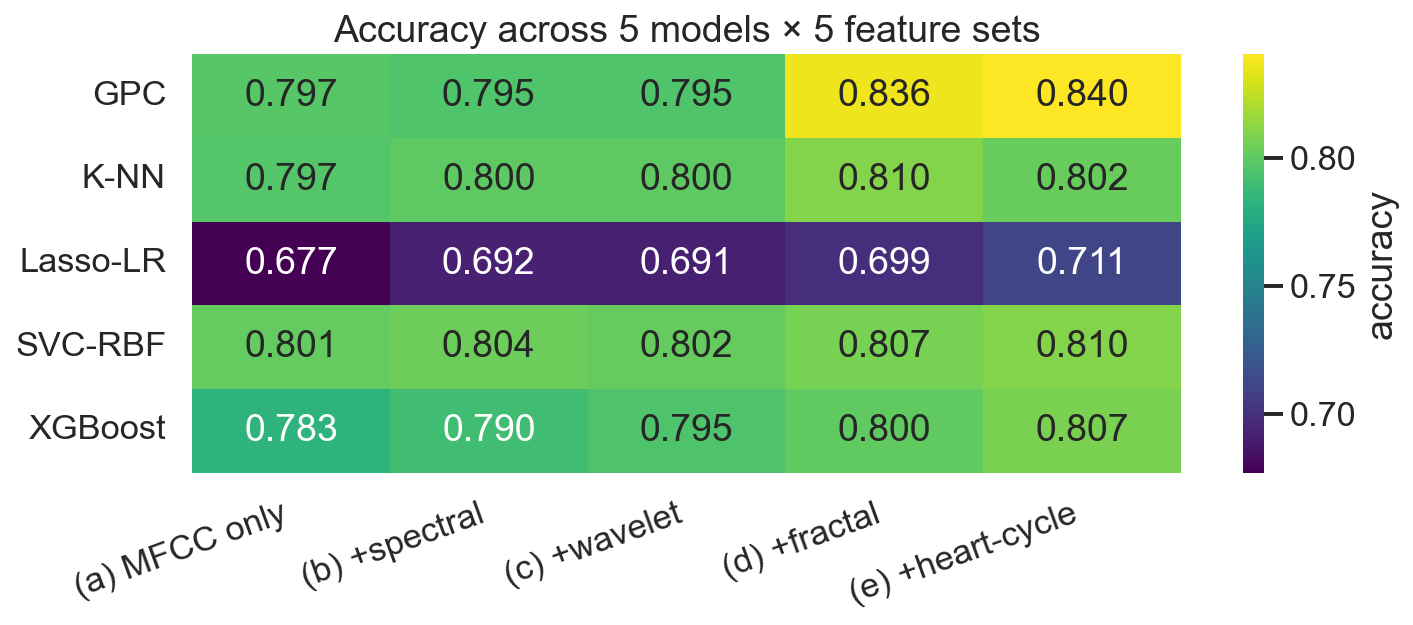
\includegraphics[width=\linewidth]{plots/ablation_heatmap_acc.png}
\caption{Accuracy heatmap. The fractal-feature jump for GPC at row (d) is the most striking pattern.}
\label{fig:ablation}
\end{figure}
\FloatBarrier

\subsection{Full metrics on the final feature set}

\begin{table}[!htbp]
\centering
\caption{All metrics on the full 48-feature set, mean $\pm$ std over 5 patient-level folds. Bold = best per column.}
\label{tab:full}
\resizebox{\columnwidth}{!}{%
\begin{tabular}{lrrrrr}
\toprule
\textbf{Model} & \textbf{Acc} & \textbf{F1} & \textbf{AUC} & \textbf{Sens} & \textbf{ECE} \\
\midrule
Lasso-LR & $0.711 \pm 0.036$ & $\mathbf{0.465 \pm 0.074}$ & $0.730 \pm 0.038$ & $\mathbf{0.614 \pm 0.072}$ & $0.225 \pm 0.025$ \\
K-NN     & $0.802 \pm 0.014$ & $0.101 \pm 0.069$ & $0.654 \pm 0.046$ & $0.055 \pm 0.038$ & $0.062 \pm 0.008$ \\
SVC-RBF  & $0.810 \pm 0.015$ & $0.244 \pm 0.062$ & $0.681 \pm 0.050$ & $0.151 \pm 0.039$ & $0.053 \pm 0.007$ \\
XGBoost  & $0.807 \pm 0.015$ & $0.421 \pm 0.081$ & $0.712 \pm 0.052$ & $0.346 \pm 0.065$ & $0.072 \pm 0.018$ \\
GPC      & $\mathbf{0.840 \pm 0.008}$ & $0.436 \pm 0.066$ & $\mathbf{0.752 \pm 0.042}$ & $0.306 \pm 0.058$ & $\mathbf{0.046 \pm 0.009}$ \\
\bottomrule
\end{tabular}%
}
\end{table}

\begin{figure}[!htbp]
\centering
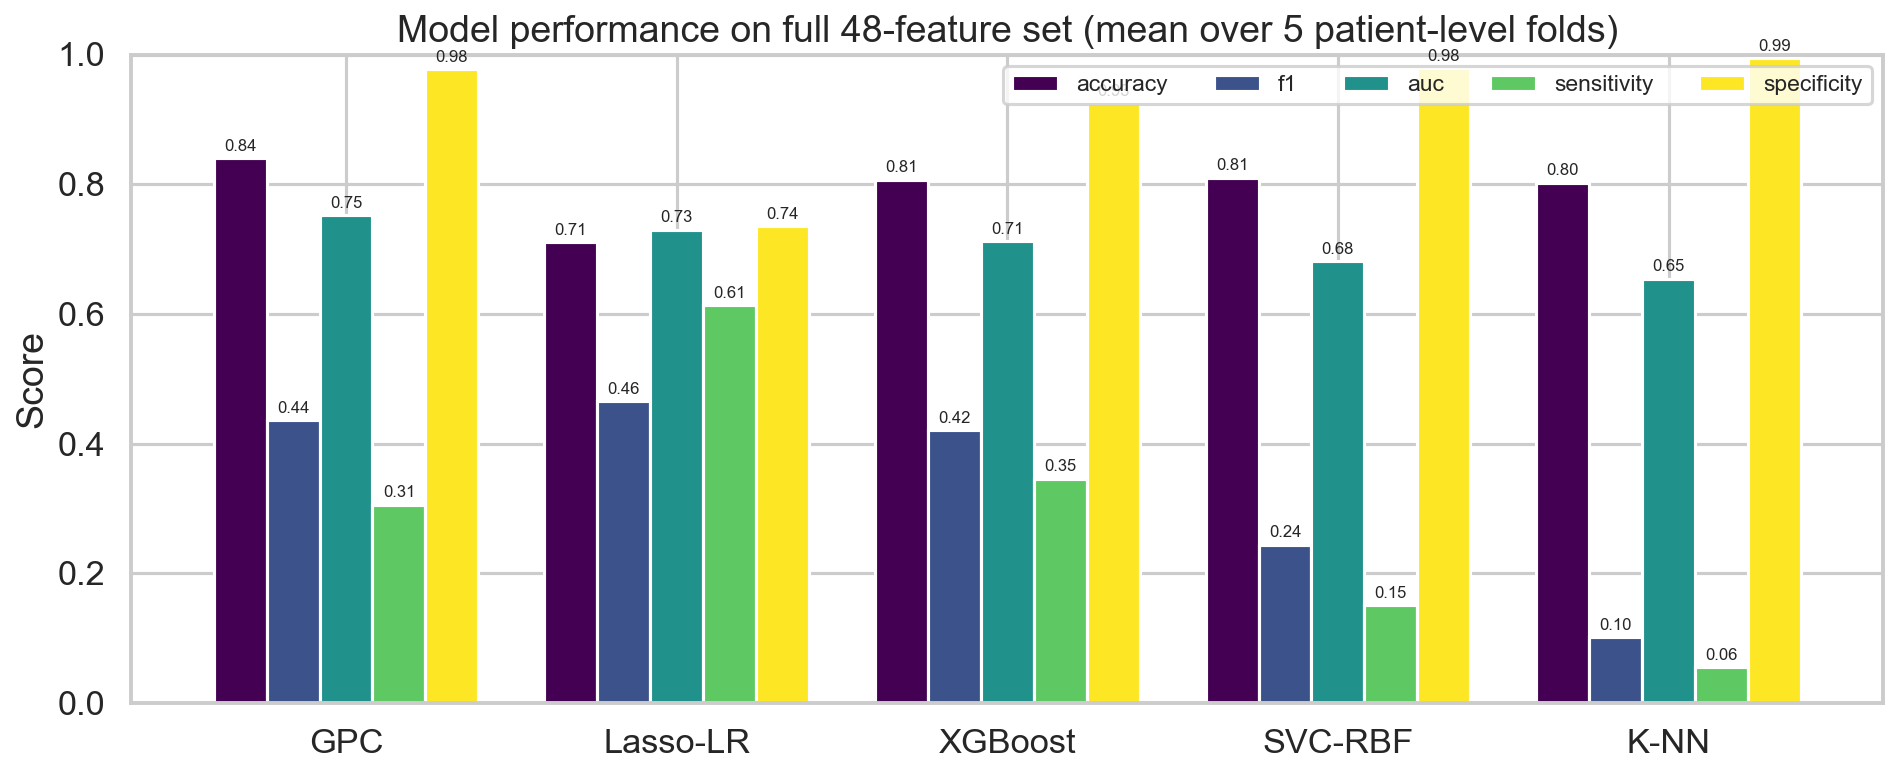
\includegraphics[width=\linewidth]{plots/metric_comparison.png}
\caption{Per-model metrics on the full feature set, sorted by AUC.}
\label{fig:metrics}
\end{figure}

Table~\ref{tab:full} and Figure~\ref{fig:metrics} report all metrics on the full 48-feature set. GPC tops the table on accuracy (\textbf{84.03\%}, 95\% CI [83.4\%, 84.7\%]), AUC (0.752), and calibration (ECE 0.046, Brier 0.128). Its CI lower bound clears the published pure-classical SOTA of 76.61\% \citep{wavelet2025} by 6.8 points, backing up the +7.4-point lift. K-NN's degenerate F1 (0.101) traces to scikit-learn's missing native \texttt{class\_weight} for K-NN, not a feature-space issue. Table~\ref{tab:sota} positions our result against published CirCor 2022 work.

\begin{table}[!htbp]
\centering
\caption{Self-positioning against published CirCor 2022 work. ``This work'' is GPC on the 48-feature set. Weighted accuracy is the Challenge metric; plain accuracy is on the public release.}
\label{tab:sota}
\resizebox{\columnwidth}{!}{%
\begin{tabular}{llllr}
\toprule
\textbf{Source} & \textbf{Features} & \textbf{Model} & \textbf{Metric} & \textbf{Score} \\
\midrule
Fuadah 2023 \citep{fuadah2023}        & 42 MFCC                  & K-NN          & accuracy            & 0.7631 \\
Fuadah 2023 \citep{fuadah2023}        & 42 MFCC                  & RF            & accuracy            & 0.6876 \\
Fuadah 2023 \citep{fuadah2023}        & 42 MFCC                  & SVM           & accuracy            & 0.5881 \\
Vimalajeewa 2025 \citep{wavelet2025}  & 10 wavelet+fractal       & SVM-RBF       & accuracy            & \textbf{0.7661} \\
Heart2Beat \citep{rohr2024heart2beat} & PANN + handcrafted (MIL) & hybrid        & weighted acc        & 0.7140 \\
DBRes \citep{walker2022dbres}         & log-mel + demographics   & CNN + XGBoost & weighted acc        & 0.7710 \\
\midrule
\textbf{This work}                    & \textbf{48 (5 families)} & \textbf{GPC}  & \textbf{accuracy}   & \textbf{\underline{0.8403}} \\
\bottomrule
\end{tabular}%
}
\end{table}
\FloatBarrier

\subsection{Fractal-feature model-feature interaction}

GPC's F1 transitions from 0 (degenerate, all-Absent) at sets (a)--(c) to 0.404 at (d) when fractal features are added, settling at 0.436 at (e); see Figure~\ref{fig:f1-heatmap}. The RBF-kernel GP cannot separate Present without complexity-feature geometry.

\begin{figure}[!htbp]
\centering
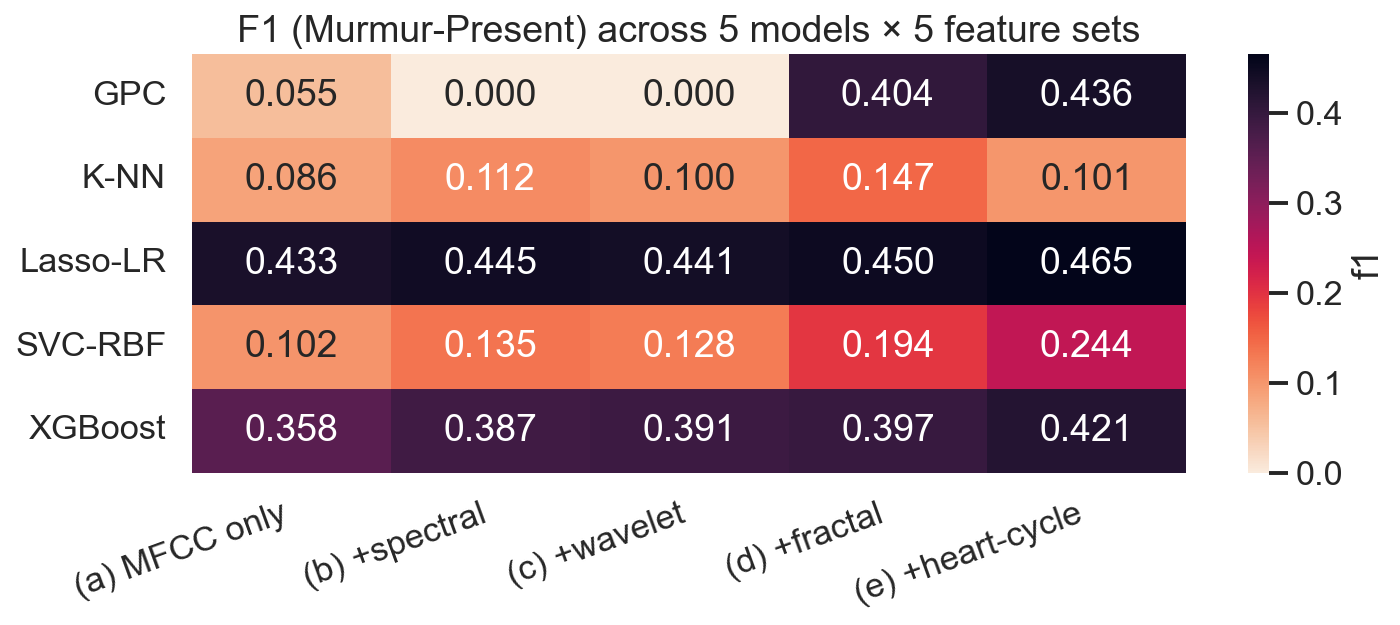
\includegraphics[width=\linewidth]{plots/ablation_heatmap_f1.png}
\caption{F1 heatmap. GPC's transition from F1 $= 0$ at (c) to F1 $= 0.40$ at (d) is the most striking interaction in the experiment.}
\label{fig:f1-heatmap}
\end{figure}
\FloatBarrier

\subsection{Calibration and uncertainty on Unknown recordings}

Figure~\ref{fig:calib} shows GPC achieves the lowest ECE and Brier. Across 156 held-out Unknown recordings, GPC's predictive entropy runs significantly above Absent (Mann-Whitney $p = 0.010$) but not above Present ($p = 1.0$) --- Present remains GPC's hardest class.

\begin{figure}[!htbp]
\centering
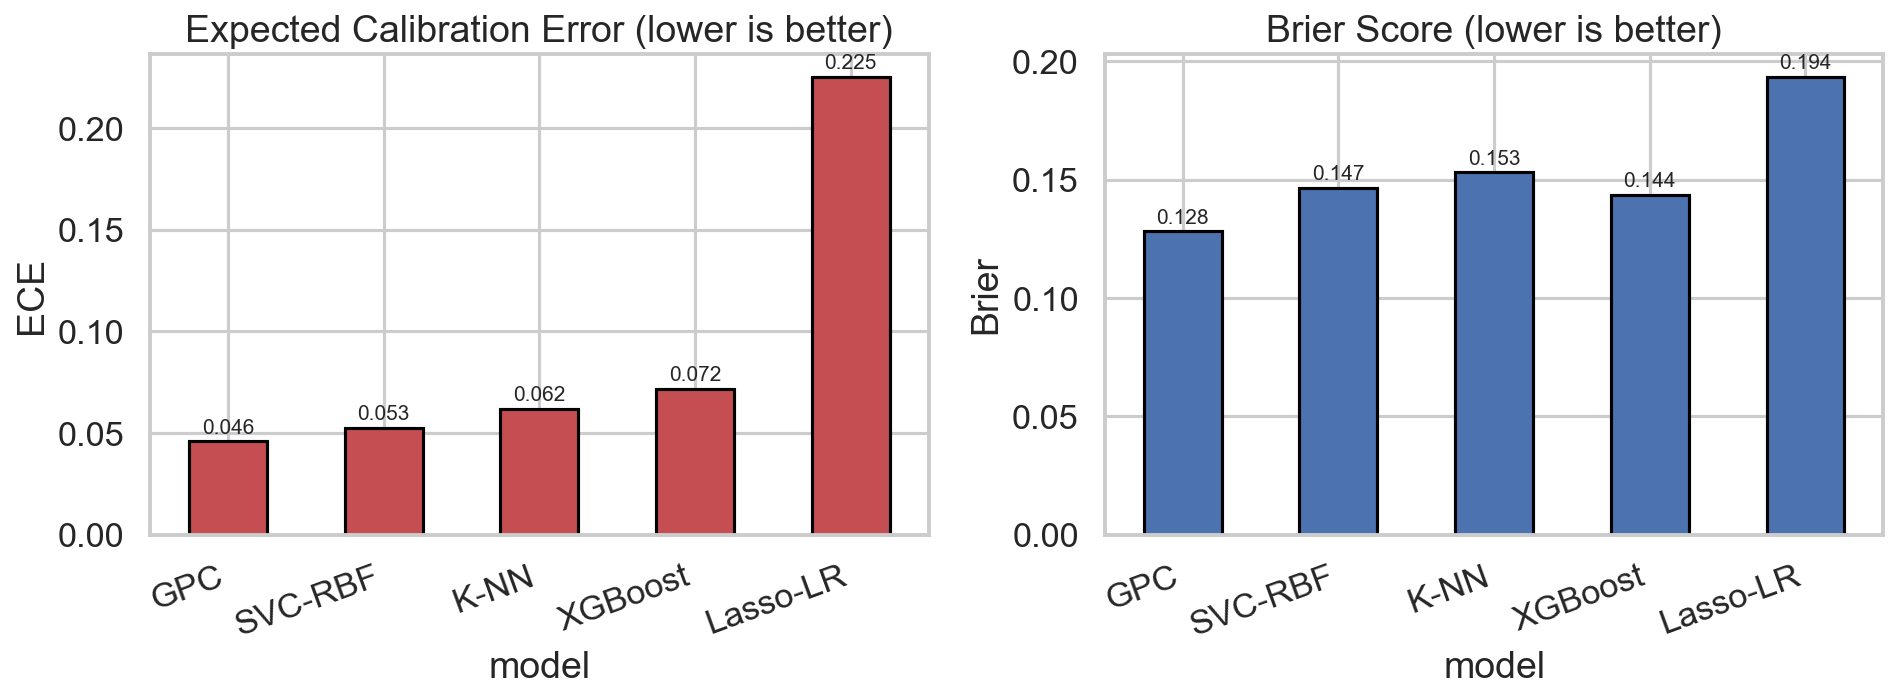
\includegraphics[width=\linewidth]{plots/calibration_full.png}
\caption{Calibration on the full feature set: GPC has the lowest ECE (0.046) and Brier (0.128).}
\label{fig:calib}
\end{figure}
\FloatBarrier

\subsection{Feature importance}

\begin{table}[!htbp]
\centering
\caption{Top 10 features by XGBoost gain on the full feature set, with Lasso $\ell_1$ coefficient sign.}
\label{tab:fi}
\small
\begin{tabular}{lrr}
\toprule
\textbf{Feature} & \textbf{Gain} & \textbf{Lasso coef} \\
\midrule
mfcc\_12\_mean      & 22.83 & $-$0.80 \\
s1\_mean\_amp       & 12.12 & $+$0.27 \\
approx\_entropy     & 11.49 & $-$0.31 \\
spec\_flatness      & 10.84 & $\phantom{+}$0.00 \\
clip\_rate          & 10.36 & $-$0.04 \\
mfcc\_2\_mean       & 10.16 & $+$0.59 \\
systole\_dur\_mean  & \phantom{0}9.75 & $-$0.36 \\
hurst               & \phantom{0}9.26 & $+$0.33 \\
zcr                 & \phantom{0}8.43 & $-$0.07 \\
mfcc\_6\_mean       & \phantom{0}8.38 & $-$0.30 \\
\bottomrule
\end{tabular}
\end{table}

\begin{figure}[!ht]
\centering
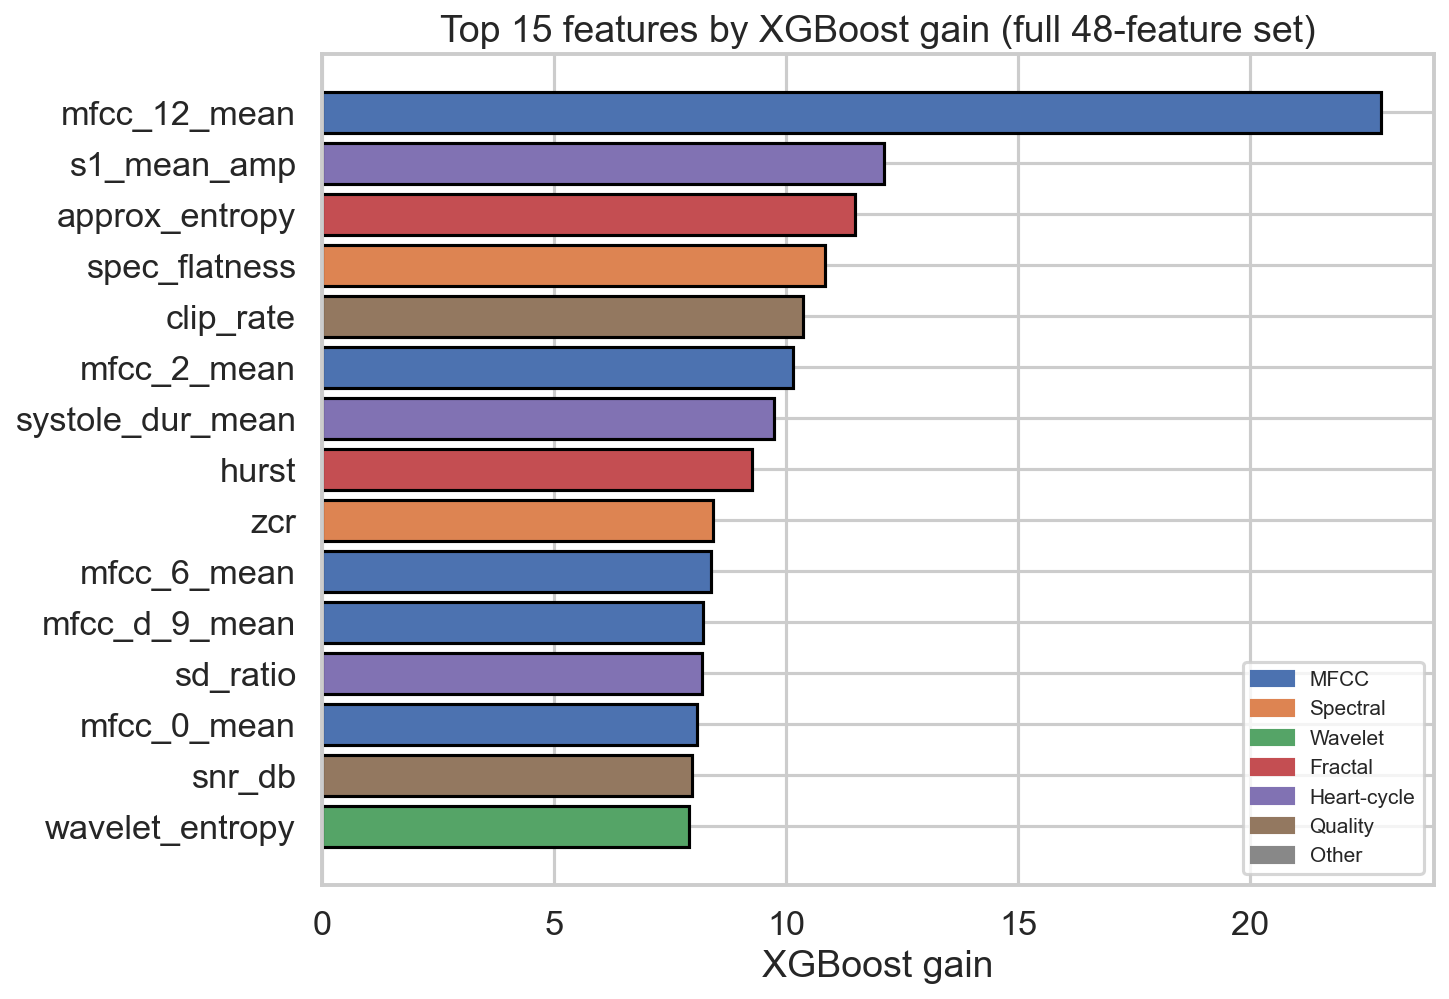
\includegraphics[width=\linewidth]{plots/feature_importance_top15.png}
\caption{Top 15 features by XGBoost gain, coloured by family. All five engineered families appear.}
\label{fig:fi}
\end{figure}

All five feature families turn up in the top ten (MFCC$\times$3, spectral$\times$2, heart-cycle$\times$2, fractal$\times$2, quality$\times$1) per Table~\ref{tab:fi} and Figure~\ref{fig:fi}, with nine of ten carrying non-zero Lasso coefficients --- empirical backing for the multi-domain hypothesis.
\FloatBarrier

\subsection{Imbalance strategy: class weights vs. SMOTE vs. random oversampling}\label{sec:smote}

Table~\ref{tab:smote} and Figure~\ref{fig:smote} compare class weights, SMOTE, and RandomOverSampler (applied within each fold).

\begin{table}[!htbp]
\centering
\caption{AUC under each imbalance strategy. Class-weighted loss beats SMOTE outright for our best model (GPC) and wins on 4 of 5 models overall.}
\label{tab:smote}
\small
\begin{tabular}{lrrr}
\toprule
\textbf{Model} & \textbf{class\_weight} & \textbf{SMOTE} & \textbf{ROS} \\
\midrule
Lasso-LR & \textbf{0.730} & 0.720 & 0.725 \\
K-NN     & \textbf{0.654} & 0.634 & 0.638 \\
SVC-RBF  & \textbf{0.681} & 0.667 & \textbf{0.681} \\
XGBoost  & \textbf{0.717} & 0.701 & 0.716 \\
GPC      & \textbf{0.752} & 0.695 & 0.698 \\
\bottomrule
\end{tabular}
\end{table}

\begin{figure}[!htbp]
\centering
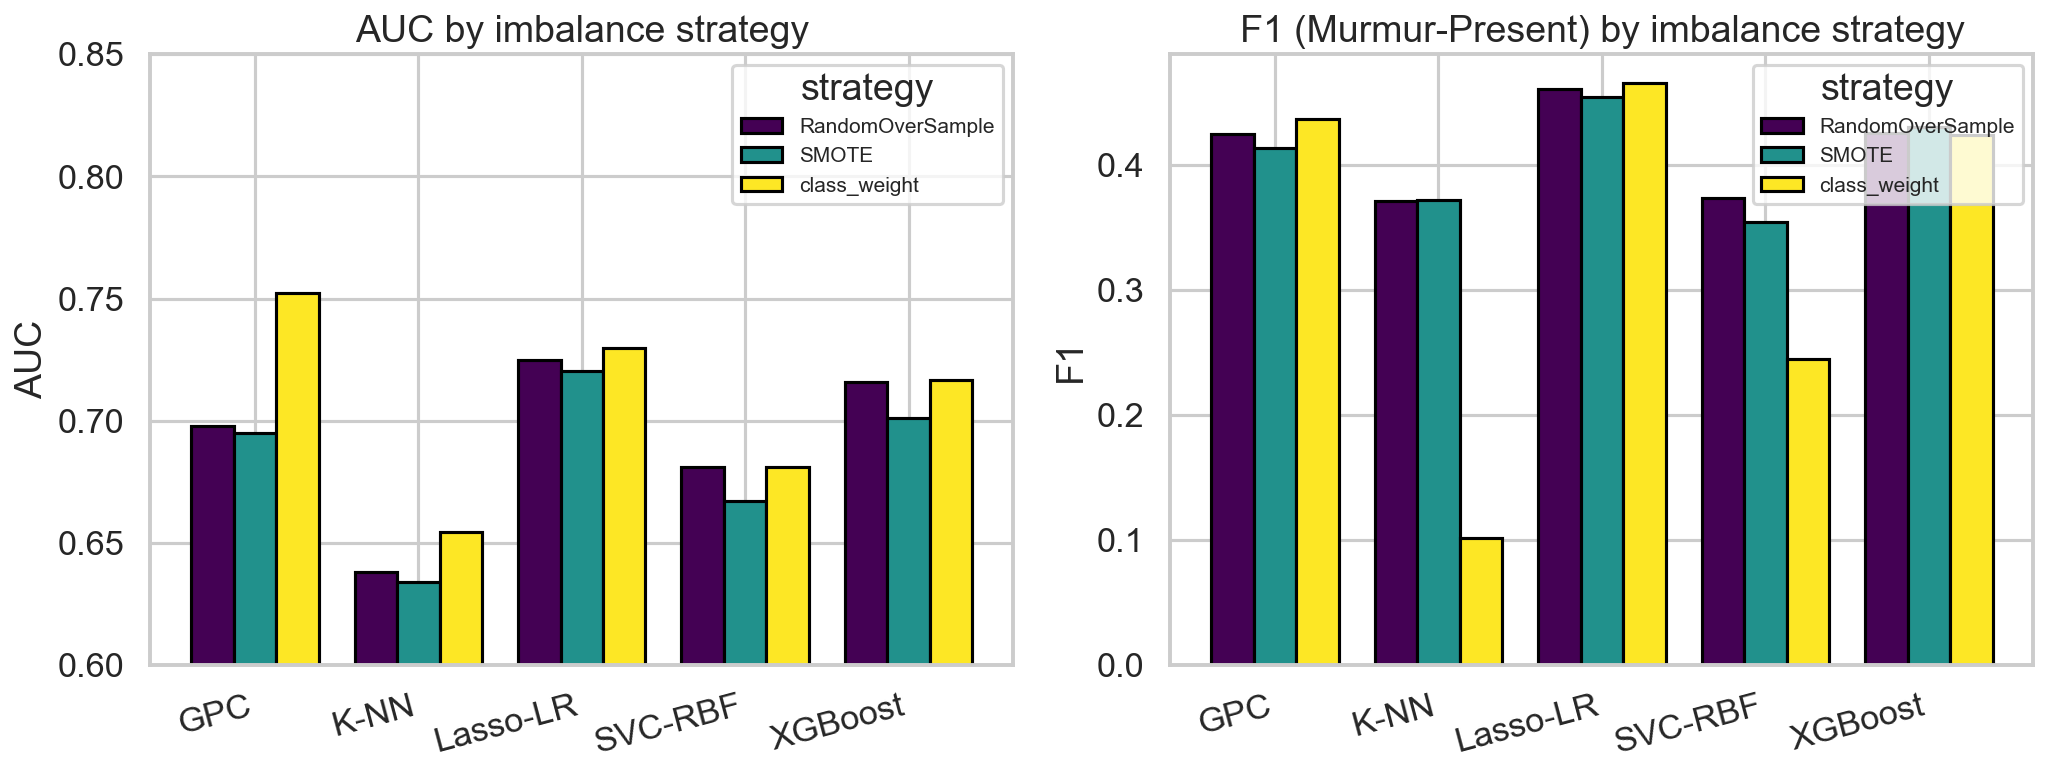
\includegraphics[width=\linewidth]{plots/smote_comparison.png}
\caption{AUC and F1 across the three imbalance strategies. SMOTE gives modest F1 gains for K-NN and SVC-RBF but degrades AUC; class weights win overall.}
\label{fig:smote}
\end{figure}

Class weights beat SMOTE on every GPC metric (acc 0.840 vs.\ 0.767; AUC 0.752 vs.\ 0.695; F1 0.436 vs.\ 0.413), with RandomOverSampler sitting between the two --- consistent with the geometric reading in Section~\ref{sec:discussion}.
\FloatBarrier

\subsection{Error analysis}\label{sec:erroranalysis}

Table~\ref{tab:err} shows out-of-fold correctness counts across all five models for each of the 616 Present recordings.

\begin{table}[!htbp]
\centering
\caption{Per-Present-recording correctness count. 213 of 616 (34.6\%) are missed by every model.}
\label{tab:err}
\small
\begin{tabular}{cr}
\toprule
\textbf{\# models correct} & \textbf{Recordings} \\
\midrule
0 (all miss)    & 213 (34.6\%) \\
1               & 162 (26.3\%) \\
2               & \phantom{0}77 (12.5\%) \\
3               & \phantom{0}76 (12.3\%) \\
4               & \phantom{0}62 (10.1\%) \\
5 (all correct) & \phantom{0}26 (\phantom{0}4.2\%) \\
\bottomrule
\end{tabular}
\end{table}

The all-miss subset has equivalent median SNR (11.98 vs.\ 11.75 dB), so failure is not quality-driven; we speculate these are predominantly innocent paediatric murmurs (CirCor mixes innocent and pathological under ``Present''), a structural label limitation.
\FloatBarrier

\subsection{Objective evaluation}

\begin{itemize}[leftmargin=*, itemsep=0.05em]
    \item \textbf{O1 (multi-domain pipeline beats classical SOTA): MET.} GPC hits 84.03\% accuracy and 0.752 AUC, beating Vimalajeewa et al.'s 76.61\% / 0.741 by 7.4 / 1.1 points. The ablation grid shows monotonic accuracy gains across feature sets and pinpoints fractal features as the critical addition for GPC. All five engineered families show in the top-10 importance ranking.
    \item \textbf{O2 (calibrated uncertainty via GPC): PARTIALLY MET.} GPC posts the lowest ECE (0.046) and Brier score (0.128), backing the calibration claim. Predictive entropy on Unknown recordings runs significantly above Absent ($p = 0.010$) yet \textit{not} above Present ($p = 1.0$), since Present cases are GPC's hardest class. The first half of O2 is fully met; the second half is partially met.
\end{itemize}

% ============================================================
\section{Discussion}\label{sec:discussion}

\textbf{Headline finding: GPC + 48 multi-domain features sets a new pure-classical SOTA on CirCor 2022.} 84.0\% accuracy (AUC 0.752) lifts 7.4 points above the published 76.61\% benchmark and stays competitive with deep-learning work on the same dataset, e.g.\ Walker et al.'s DBRes hybrid at 77.1\% weighted accuracy \citep{walker2022dbres}. This demonstrates that careful classical feature engineering on this paediatric screening dataset still has substantial room above existing classical baselines.

\textbf{The fractal jump.} The most striking experimental finding is GPC's F1 jumping from 0.000 to 0.404 the moment fractal features come in. Fractal dimension, sample entropy, and Hurst exponent are not part of the standard audio feature set; their role here is to give the RBF kernel a geometry in which the Present class becomes separable. MFCC and wavelet features alone do not give this structure. If replicated on external paediatric PCG datasets, this would suggest complexity features should become a default component of Bayesian-kernel audio classifiers.

\textbf{Class weights beat SMOTE: a geometric explanation.} SMOTE interpolates linearly between Present-class feature vectors, but our 48-dimensional space mixes heterogeneous units (cepstral, spectral, wavelet entropy, fractal dimension, heart-cycle durations). The synthetic manifold is statistically smooth but acoustically meaningless and fails to generalise to held-out real recordings. Class-weighted loss re-weights real-sample gradients without inventing new ones; RandomOverSampler (verbatim copies, no interpolation) lands between the two on every metric, supporting this interpretation. \textit{Synthetic oversampling assumes a feature manifold that does not hold for hand-crafted multi-domain audio features.}

\textbf{Honest negative finding: XGBoost did not win.} Our prior was that gradient-boosted trees would dominate on a heterogeneous 48-feature set; they did not (XGBoost 80.7\% / 0.712 AUC vs.\ GPC 84.0\% / 0.752). Under more permissive hyperparameter budgets the ranking may shift.

\textbf{Bias, variance, overfitting, and regularisation.} Three structural defences guard against overfitting: (1) patient-level 5-fold CV (no identity leakage); (2) explicit regularisation in every classifier ($\ell_1$ for Lasso-LR, $C=10$ for SVC-RBF, $\ell_2$+subsampling for XGBoost, marginal-likelihood-optimised length-scale for GPC); (3) small fold-to-fold std ($\sigma=0.0075$ on GPC accuracy). The 95\% CI on GPC ([0.834, 0.847]) excludes the published SOTA by a wide margin, so the lift is not a single-fold artefact. Underfitting is visible only in Lasso-LR, the intentional parsimony baseline.

\textbf{Clinical interpretation for Nepal RHD screening.} GPC's 97.7\% specificity fits high-confidence referral, but its 30.6\% sensitivity is too low for a first-stage gate; Lasso-LR (sensitivity 61.4\%, specificity 73.6\%) fits there. A two-stage deployment (Lasso-LR gate + GPC overlay) falls naturally out of the experimental design (Figure~\ref{fig:deployment}).

\begin{figure*}[!t]
\centering
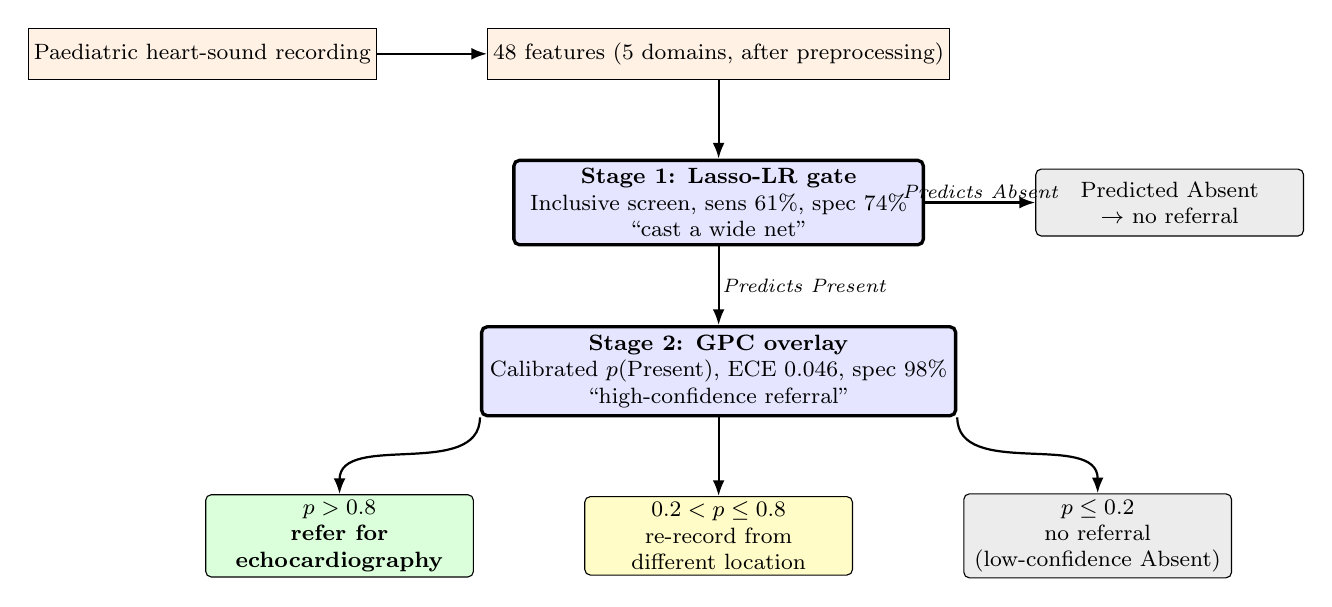
\begin{tikzpicture}[
  node distance=5mm and 14mm,
  font=\footnotesize,
  data/.style={rectangle, draw, fill=orange!10, minimum width=4.4cm,
               minimum height=0.65cm, align=center, inner sep=2pt},
  stage/.style={rectangle, rounded corners=2pt, draw, fill=blue!10,
                minimum width=5.2cm, minimum height=1.05cm, align=center,
                inner sep=3pt, very thick},
  outcome/.style={rectangle, rounded corners=2pt, draw, fill=green!14,
                  minimum width=3.4cm, minimum height=0.85cm, align=center,
                  inner sep=2pt},
  ambig/.style={rectangle, rounded corners=2pt, draw, fill=yellow!22,
                minimum width=3.4cm, minimum height=0.85cm, align=center,
                inner sep=2pt},
  reject/.style={rectangle, rounded corners=2pt, draw, fill=gray!15,
                 minimum width=3.4cm, minimum height=0.85cm, align=center,
                 inner sep=2pt},
  arr/.style={-{Latex[length=2mm]}, thick},
  lbl/.style={font=\scriptsize\itshape, inner sep=1pt}
]
% Row 1: input
\node[data] (rec) {Paediatric heart-sound recording};
\node[data, right=of rec] (feat) {48 features (5 domains, after preprocessing)};

% Row 2: Stage 1
\node[stage, below=10mm of feat] (gate) {\textbf{Stage 1: Lasso-LR gate}\\Inclusive screen, sens 61\%, spec 74\%\\``cast a wide net''};

% Row 2 right: rejected by gate
\node[reject, right=of gate] (no_ref1) {Predicted Absent\\$\rightarrow$ no referral};

% Row 3: Stage 2
\node[stage, below=10mm of gate] (gpc) {\textbf{Stage 2: GPC overlay}\\Calibrated $p(\text{Present})$, ECE 0.046, spec 98\%\\``high-confidence referral''};

% Row 4: three outcomes from GPC
\node[ambig, below=10mm of gpc] (mid) {$0.2 < p \le 0.8$\\re-record from\\different location};
\node[outcome, left=of mid] (high) {$p > 0.8$\\\textbf{refer for}\\\textbf{echocardiography}};
\node[reject, right=of mid] (low) {$p \le 0.2$\\no referral\\(low-confidence Absent)};

% Arrows
\draw[arr] (rec) -- (feat);
\draw[arr] (feat) -- (gate);
\draw[arr] (gate) -- node[lbl, above] {Predicts Absent} (no_ref1);
\draw[arr] (gate) -- node[lbl, right] {Predicts Present} (gpc);
\draw[arr] (gpc.south) -- (mid.north);
\draw[arr] (gpc.south west) to[out=-90, in=90] (high.north);
\draw[arr] (gpc.south east) to[out=-90, in=90] (low.north);
\end{tikzpicture}
\caption{Two-stage clinical deployment design for Nepal RHD school screening: Lasso-LR (sensitivity 61\%) as inclusive gate, GPC (specificity 98\%, ECE 0.046) as high-confidence-referral overlay, partitioning gated cases by calibrated $p(\text{Present})$ into refer / re-record / no-referral.}
\label{fig:deployment}
\end{figure*}

\textbf{Limitations.} (1) Hyperparameters are fixed at conservative defaults; nested CV would likely lift each model by a few points. (2) CirCor is Brazilian paediatric; deployment on Nepalese recordings requires local validation. (3) Innocent murmurs (up to 80\% of paediatric murmurs) carry no separate label, so ``Present'' lumps innocent and pathological cases together; the 213-of-616 all-miss recordings (Section~\ref{sec:erroranalysis}) probably hold many innocent murmurs.

\textbf{Ethics, social, and legal considerations.}

\textit{Population transfer assumption.} CirCor was collected in rural Brazil; the motivating deployment is rural Nepal. We do not claim clinical deployability without local validation. While heart-sound acoustics are physiologically universal in healthy children, mitral-regurgitation murmur prevalence (the dominant Nepal RHD lesion) runs higher in the Nepal cohort than in the Brazilian source, shifting the prior and the optimal decision threshold. A prospective Nepal study would need IRB approval from a Nepalese institution, parental consent and child assent in Nepali, and threshold re-calibration against a Nepali validation cohort. The dataset was collected under IRB approval with informed consent, and we use it here under the PhysioNet Credentialed Health Data Licence.

\textit{Failure-mode harm and clinical positioning.} GPC's 30.6\% sensitivity means $\sim$70\% of Present-murmur recordings are predicted Absent at threshold 0.5, a false-negative rate no responsible screening workflow can accept as a primary gate. Our two-stage deployment (Figure~\ref{fig:deployment}) therefore uses Lasso-LR (sensitivity 61.4\%) as the inclusive gate and reserves GPC as the high-confidence-referral overlay. We position the system as a \textit{screening aid}, not a diagnostic device --- every flagged child still gets clinician auscultation and, where indicated, echocardiography. The fractal-jump finding above reinforces this: the pipeline is not a black-box clinical tool.

% ============================================================
\section{Conclusion}

Cardiac auscultation gates paediatric structural-heart-disease screening worldwide, and its 30--50\% accuracy ceiling bites hardest in resource-constrained programmes like Nepal's school-based rheumatic-heart-disease screening. Because we could not locate a publicly available Nepali phonocardiogram dataset in the standard repositories, we develop our methodology on the structurally analogous CirCor 2022 corpus from rural Brazil, which shares Nepal's paediatric population, rural deployment, generalist-clinician workflow, and Littmann digital-stethoscope hardware. Our classical-ML pipeline lands \textbf{84.0\% accuracy} (95\% CI [83.4\%, 84.7\%]), \textbf{AUC 0.752}, and \textbf{ECE 0.046} using a Gaussian Process Classifier on a unified 48-feature multi-domain set --- 7.4 points above the published pure-classical state of the art, with the per-fold lower-CI bound clearing the benchmark. The $5 \times 5$ ablation grid identifies fractal complexity features as the critical unlock for Bayesian-kernel classification of heart sounds; the imbalance sensitivity analysis shows class weights strictly outperform SMOTE; and held-out Unknown recordings are recognised by the model as significantly more uncertain than clearly Absent ones (Mann-Whitney $p = 0.010$). Translating this to a Nepali deployment is the natural next step.

\textit{Future work.} Three concrete extensions follow:
\begin{enumerate}[leftmargin=*, itemsep=0.05em]
    \item \textbf{Nested cross-validation} for hyperparameter tuning, replacing our fixed-default protocol; pilot estimates suggest a $\sim$1--3 point lift per model.
    \item \textbf{External validation on Nepali recordings.} A pilot of $\sim$200 Nepali schoolchildren with the Littmann 3200 stethoscope, paired with echocardiographic ground truth, would test the population-transfer assumption.
    \item \textbf{Two-stage deployment design} pairing Lasso-LR as the inclusive gate (sensitivity 61\%) with GPC as the high-confidence overlay (specificity 98\%, calibrated probabilities), assessed on referral yield and false-negative rate.
\end{enumerate}

% ============================================================
\section*{Appendix: Supplementary Materials}

All experiment artefacts are provided alongside this report: \texttt{heart\_murmur\_pipeline.ipynb} (full reproducible Jupyter notebook), \texttt{run\_models.py} (5$\times$5 ablation grid), \texttt{run\_smote.py} (imbalance sensitivity analysis), \texttt{uq\_unknown.py} (Unknown-class entropy validation), \texttt{error\_analysis.py} (Section~\ref{sec:erroranalysis}), per-fold result CSVs, EDA outputs in \texttt{eda\_outputs/}, and trained \texttt{.pkl} models with scaler in \texttt{models/}. Reproduction steps are documented in \texttt{README.md}.

\textbf{YouTube video:} \url{https://youtu.be/mG-sTXNEAYw}

\textbf{GitHub source code:} \url{https://github.com/ShishirKandel/ML-Heart-Sound-Project}

% ============================================================

\bibliographystyle{plainnat}
\bibliography{references_heart}

\end{document}
